
%%%%%%%%%%%%%%%%%%%%%%% file typeinst.tex %%%%%%%%%%%%%%%%%%%%%%%%%
%
% This is the LaTeX source for the instructions to authors using
% the LaTeX document class 'llncs.cls' for contributions to
% the Lecture Notes in Computer Sciences series.
% http://www.springer.com/lncs       Springer Heidelberg 2006/05/04
%
% It may be used as a template for your own input - copy it
% to a new file with a new name and use it as the basis
% for your article.
%
% NB: the document class 'llncs' has its own and detailed documentation, see
% ftp://ftp.springer.de/data/pubftp/pub/tex/latex/llncs/latex2e/llncsdoc.pdf
%
%%%%%%%%%%%%%%%%%%%%%%%%%%%%%%%%%%%%%%%%%%%%%%%%%%%%%%%%%%%%%%%%%%%


\documentclass[runningheads,a4paper]{llncs}

\usepackage[a4paper, total={7in, 8in}]{geometry}
\usepackage[margin=1cm]{caption}

\usepackage{amssymb}
\setcounter{tocdepth}{3}
\usepackage{graphicx}
\usepackage{subcaption}
\usepackage{listings}
%\lstset{
%	numbers=left
%	language=Java
%	frame=single,
%	breaklines=true,
	%postbreak=\raisebox{0ex}[0ex][0ex]{\ensuremath{\color{red}\hookrightarrow\space}}
%}
\renewcommand{\lstlistingname}{Code}

\captionsetup{compatibility=false}

\usepackage{url}
\urldef{\mailsa}\path|{alfred.hofmann, ursula.barth, ingrid.haas, frank.holzwarth,|
\urldef{\mailsb}\path|anna.kramer, leonie.kunz, christine.reiss, nicole.sator,|
\urldef{\mailsc}\path|erika.siebert-cole, peter.strasser, lncs}@springer.com|    
\newcommand{\keywords}[1]{\par\addvspace\baselineskip
\noindent\keywordname\enspace\ignorespaces#1}

\begin{document}

\mainmatter  


\newpage
\tableofcontents
\newpage

\abstract{
This assignment is about ``TinyCoin: Simulating fraudolent mining strategies in a simplified Bitcoin Network'', the final project in Peer to peer systems course at University of Pisa. 
In this project, the simulation of TinyCoin is implemented with two different strategies (normal and selfish~\cite{eyal2014majority} ways). The Aim of the project is to find the number of fork and the total time need to solve it.
Because of the variety of the information, the project is experimented with different parameters such as: the percentage of selfish miners in total of honest miner created randomly, the power of selfish miners, the latency between two blocks and the latency of the network. 
However, other parameters also can need to consider: the number of nodes in the network, the degree or the connections between nodes.
} 

\section{Introduction}
\label{Intro}
% concept of block chain
% concept 
% describe basic idea of the project

With the development of technology, nowadays there are a lot of cryptocurrency and one of the most popular cryptocurrency is Bitcoin. 
Each of user joining the Bitcoin network has a public log called block chain.
This block chain is a list of blocks in each of which another list of transactions is stored.
To make the security of the block chain, a chain of cryptographic puzzles which is solved by some users called miners is utilized.
When a miner solves a cryptopuzzle, it can create a new block containing a set of transaction and then take the rewards.
Therefore, the goal of miners is about trying to solve cryptopuzzles, but to solve it the miners need to have a lot of resources or a powerful computation, which supports miners in increasing the probability resolving a cryptopuzzle.
In addition, the Bitcoin needs a large number of honest miners who correctly follow the rules of Bitcoin protocol.

In the assignment, another cryptocurrency is used to make a simulation called Tinycoin whose idea is also similar to the simple Bitcoin's idea, but it eliminates some parts.
Furthermore, another strategy is applied to consider the different from the honest strategy made by honest miners.
The new strategy is called selfish strategy and based on the paper~\cite{eyal2014majority}.
With the diversity of parameters not only from the network but also from Tinycoin protocol, the simulation utilizes a list of parameters such as: the number of nodes in the network, the number of degree of each node, the percentage of selfish miner in the total miners, the power of selfish miners, the time of generation of two blocks and the latency of block propagation.
Based on these parameters, the purpose of the simulation is to consider about the number of forks generated and the total time consuming to solve these forks.

The remaining of the assignment is followed: Section~\ref{CA} describes about selfish pool and its algorithm, the simulation is showed in Section~\ref{TS} and two last Section~\ref{Exper} and Section~\ref{Con} represent about the experiments and conclusion, respectively.

\section{Selfish Miner}
\label{CA}
% explain sth from the paper
The Bitcoin is considered a technique which is equitable to its participants. Therefore, the reward is believed that it is shared based on the resource of members in the pool.
Nevertheless, in the paper~\cite{eyal2014majority}, this wrong conventional wisdom is explained and then a strategy to exploit it called selfish strategy is described.
Miners who follow the selfish strategy is called selfish miners.

The basic idea of this strategy is about keeping new blocks in a private and forking the public block chain.
Whereas the honest miners try to mine a new block on the public block chain, the selfish nodes mine on its private chain.
It hence exists two situations which can be:
\begin{itemize}
\item One of them is the case in which the private pool creates a lot of new blocks and continues keeping them in the private.
\item Another case is that when the public reaches the length which is equal to the length of the private block chain, the private publishes blocks to public.
\end{itemize}

The analysis from the paper~\cite{eyal2014majority} shows that selfish and honest miners spend an amount of resources on mining cryptopuzzles, but the selfish miners will earn more reward than honest miners while the honest miners waste more resources than other selfish miners.
After that, the selfish pool can be appealing honest miners who will change the behavior and participate the selfish pool.
As the result, the selfish pool will dominate and stop the decentralization of the currency.
To reach this goal, the paper~\cite{eyal2014majority} mentions about a threshold size of selfish mining pool. If the selfish pool exceeds this threshold, the Bitcoin system will be in a threat.
After experiments, the paper concludes that the Bitcoin will be not safe if existing a selfish mining pool contains more than one third of the total power of the network, which means the selfish pool can be capable to get rewards more than the resources which is spent by this pool.

\begin{lstlisting}[numbers=left,language=Java,frame=single,breaklines=false,label=SelfishAlgorithm, caption= Selfish-Mine algorithm~\cite{eyal2014majority}.]
on Init
 publicChain <- publicly known blocks
 privateChain <- publicly known blocks
 privateBranchLen <- 0
 Mine at the head of the privateChain.

on My pool found a block
 DeltaPrev <- length(privateChain) - length(publicChain)
 append new block to private chain
 privateBranchLen <- privateBranchLen + 1
 if DeltaPrev = 0 and privateBranchLen = 2 
  then 
   (Was tie with branch of 1)
   publish all of the private chain 
   (Pool wins due to the lead of 1)
   privateBranchLen <- 0
 Mine at the new head of the private chain.

on Others found a block
 DeltaPrev <- length(privateChain) - length(publicChain)
 append new block to publicChain
 if DeltaPrev = 0 
  then 
   private chain<-public chain (they win)
   privateBranchLen <- 0
 else if DeltaPrev = 1 
  then 
   publish last block of the privateChain 
   (Now same length. Try our luck)
 else if DeltaPrev = 2 
  then
   publish all of the privateChain 
   (Pool wins due to the lead of 1)
   privateBranchLen <- 0
 else DeltaPrev > 2
   publish first unpublished block in private block.
 Mine at the head of the private chain.
\end{lstlisting}


Let assume that existing public and private chains and the length of private chain is greater than the length of public chain.
Hence, the honest miner mine the the shorter chain (public chain), while the selfish miners mine the longer chain (private chain).
Because of the less computation of the total mining power in selfish miners, the public chain will reach the length close to the private chain, which means the private chain cannot be always ahead of the chain.
In this situation, the private chain publishes blocks in its chain to the public.
At this case, the honest miners waste their computation and move to a new received block from the private chain.

The behavior of the selfish miners is presented by the Algorithm~\ref{SelfishAlgorithm}.
The strategy is depended on the length of the private chain versus the public chain.
Hence, there are some situations which can be considered.

When the public chain is longer than the private chain because the powers are different between them, the probability of selfish miners overtake the public chain is quite small. 
As a result, the selfish miners have to get the public chain and mine from this chain.
In case the honest miners find a new block and publish it, the selfish miners update and continue mining at the public chain.

When the selfish miners find a new block, instead of publishing this block to the public and spreading this block to other miners,
the selfish miner will keep it in its private block chain.
In the next step, there are two possible cases which can be considered: the honest miners find a new block on the public block chain which leads to the equal to the length of the private chain
or the selfish miners continue finding another new block and extend its private chain.

In the first case, when a honest miner finds a new block and makes the length of public chain being equal to the length of private chain. At this situation, the private chain immediately publishes it private block.
Thus, the selfish miners add and extend the received block from the honest miners, while the honest miners will choose a block to continue mining, which depends on the propagation.
In case of selfish miners who want to mine from the received block from honest miners, the private chain will publish another block to enjoy the rewards from both of them.
After a private block published by private chain, if the honest miners find a new block, the private pool will get the revenue of the block whereas the honest get the revenue from their block.
Another case is that if the honest miners continue mining a block from their block, they will totally get the revenue of their blocks and the private pool cannot get anything.

Another case in which a selfish miner finds a second private block. 
Then the private chain will continue leading the chain.
As a result, the selfish miners go on mining from this private chain.
The private chain will publish its first private block in case of receiving another block from honest miners.
Because of the less power of computation from selfish miners, the private chain cannot always lead the chain.
With this reason, when the public chain needs only one block to reach the private chain, the private chain publishes all of its blocks.	

\section{Tinycoin Simulation}
\label{TS}
In this part, the simulation is described based on two other small pieces. First subsection is a short explanation of PeerSim~\cite{jesi2005peersim} frame work and the general idea in the simulation. Another one is about the specific Tinycoin structure and the way it work.

\subsection{The Interaction of PeerSim in Tinycoin Simulation}
The simulation of the assignment is based on the event-based engine PeerSim frame work~\cite{jesi2005peersim} from the University of Bologna.
With this frame work, the properties of Peer-to-peer system (the nodes be added and removed continuously) can be experimented and become an easier task~\cite{jesi2005peersim}.

Because of this advantages of PeerSim, the project is built based on the frame work.
Therefor, the simulation has one config ``txt'' file and other java files to construct the protocol and to control the flow of the simulation as below:
\begin{itemize}
\item ``configFile.txt'' is to set the parameters and declare which protocols, initial points and the flow of execution.
\item ``protocolTinyCoin.java'' is the definition of the new protocol.
\item ``InitTinyCoin.java'' is the initialization of the protocol.
\item ``observerTinyCoin.java'' is the observer which can take node or understand.
\item ``Oracle.java'' is the thing which chooses a next node creating a new block.
\item ``weightedTransportTinyCoin.java'' is the definition of the weight of the network of nodes in PeerSim.
\end{itemize}

\subsubsection{Configuration File}
\label{ConfigFile}
To start the configuration ``txt'' file, in this file the general information of the network is defined such as: the number of nodes in the network, the degree of each node, the protocol is chosen, the initialization of protocol is chosen, the weight or the latency of the network, and the behavior of observer to take values depend on the requirements.
Additionally, the information of the parameters is mentioned by this file such as: the percentage of selfish miners, the power of selfish miners, the latency between two nodes and the time between.

\subsubsection{Initial Tinycoin}
At the starting point of Tinycoin protocol, each node in the network randomly has an amount of money (it is used to create transaction). The public block chain and temporary buffer are also generated the same for every node at this state. The temporary buffer is used to store some blocks which cannot find the previous block in the public block chain.

Additionally, the number and the power of miners are randomly generated, then the number of selfish miners is also created based on the parameters the percentage and the power of these selfish miners.
In more detail, after taking the number of nodes in network, this state randomly chooses some of them becoming miner nodes and also randomly set the kind of miner for these nodes.
In this simulation, four kinds of miners including: CPU, GPU, FPGA and ASIC are considered.
Thus, when a node becomes a miner, this node randomly chooses a kind of miner.
Because each kind of miner will have a different computation, the probability of different kind of miners is chosen by oracle to generate a new block in the simulation.
In more detail, the simulation considers the CPU will have one computation, GPU is two, while FPGA and ASIC being equal to each other are three.
After that from two parameters the percentage and the power of selfish miners the, number of selfish miners is generated.

\subsubsection{Oracle}
The aim of oracle is used to randomly choose a next miner who generates a new block. 
This object takes a parameter which is the time creating a new block.
Then after an amount of this time, the oracle randomly chooses a next miner.
However, the choice of oracle is based on the probability of kinds of miners, which means FPGA and ASIC have higher probability of choosing than GPU and CPU.
The reason is the probability  to become a next miner corresponds to the power or computation.

\subsubsection{Tinycoin Protocol}
The Tinycoin protocol is built based on the basic idea of the Bitcoin protocol without some parts. 
Therefore, in this protocol each node can create transactions (based on the amount of money it has) and spread it to its neighbors.
It also can create a new block in case of the miner node, otherwise it only creates transactions.
However, the protocol also considers about another strategy which is the selfish strategy~\cite{eyal2014majority}.

The processes of Tinycoin protocol for miner node is divided into two strategies that are honest and selfish strategies.
Therefore, each node follows the honest strategy or selfish strategy which depends on the definition of initial state.

In the honest strategy, each node in every cycle considers to randomly create a transaction including random two parameters a target node and an amount of money sent to this target.
However, the generation of the transaction has to be satisfied a condition which is that the amount of money sent to target is less than the total amount of money owned by this node.
Moreover, in the same cycle if this node is a miner, it will check to generate a new block or not. A node miner creates a new block in case of choosing by an Oracle. The Oracle is a object which will randomly choose a miner node to generate a new block in next cycle (The random of choosing miner is based on the power of node or the computation of node based on the kind of miners which is set from the initial step).
In case of a transaction or a block is created, this node will propagate this message to its neighbors.

When a honest miner node or a normal node is received a message (it can be a transaction or a block) from one of its neighbors, this node will check the existing of this message in the transaction pool in case of transaction message or the temporary buffer and public block chain in case of block message.
If this message exists before, this node will stop propagating this message to its neighbor, otherwise it will add this message to the transaction pool or public block chain or temporary buffer (it depends on the algorithm) and then propagate the message to its neighbors. Particularly, if the message is the transaction, it will be checked in transaction pool and in all blocks known by this node. In case of existing the transaction from the transaction pool or one of blocks known by this node, this node stops propagating the message, otherwise this transaction is added into the transaction pool.
If the received message is a block, this node will check the existing of the block in its public block chain and temporary buffer. If this block has already existed, the node will stop propagating to its neighbors, otherwise this block is added into public block chain or temporary buffer (If the previous block of the message exists on the public block chain, this message will be added into public block chain, otherwise it is added into the temporary buffer).
When a new block is added into the public block chain, each block of temporary buffer checks the new block being it previous block or not. If the new block is not its previous block, it will stay at the temporary buffer, otherwise it will be added into the public block chain and other blocks continue checking these new added blocks.

In case of selfish strategy from selfish miners, each selfish node follows the same behavior of honest, but it has another block chain called private block chain, which means these selfish nodes can generate transactions and block based on some conditions which is mentioned above.

However, in stead of adding immediately a new block created by this node into public block chain, the new block will be kept on the private block chain. 
In the simulation of the selfish miners, in stead of creating one or some private pools for some selfish miners, each selfish miner has a different private pool, which means that these selfish miners cannot share their private block chain to each other. 
Therefore, each selfish miner will publish its private block based on the algorithm~\ref{SelfishAlgorithm}.
When a new block (honest block) is sent to the selfish miner, it will add the new block into the public block chain and check the difference between the length of public block chain and private block chain.
If this difference is equal to zero, the private chain or the selfish miner loses and the private chain is assigned by the new public chain. If this difference is equal to one, which means the public and private chain are equal to each other. The private block chain will publish its last block. 
If this difference is equal to two, the selfish miner will publish all blocks in the private chain.
If this difference is greater than two, the selfish will publish the first unpublished block in private chain.

\subsubsection{Observer of Tinycoin}
The observer of Tinycoin is used to take the results (this result can be taken based on the time of execution) after executing the flow or the simulation. 
In more detail, this part takes the number of forks (the number of branches are different from the main or the longest chain) from the public Block chain of each node in the network and the time consuming to solve these forks (the amount of time is calculated based on the number of blocks which are not belong to the longest chain).
In specifically, the observer writes to a file the last result of nodes in the network, which means it counts the number of forks and the total time of solving these forks in every public block chain of each node and then takes the averages.
The way to take these results is mentioned in Section~\ref{BCS}.

\subsubsection{Weighted Transport}
The weighted transport of the network is the latency between two nodes. 
Furthermore, this part describes about the latency of the propagation of messages (block or transaction) from nodes. 
The latency of a block is depended on the number of transactions in each block.
In addition, the simulation also has a range of the latency (the min and max of the delay) to control the delay.

\subsection{Block Chain Structure in Tinycoin}
\label{BCS}
The structure block chain contains some components including transactions and blocks.
To start describing about the structure of block chain, it should be clear about the structure of its components.

\subsubsection{Transaction}
The structure of transaction has the source, destination nodes and the amount of money sent by this transaction.
Additionally, it should have a identification to recognize the transaction.

\subsubsection{Block}
The structure of block includes the identified miner, identification of the block (the identification of each block is unique) and the identification of the previous block.
In addition, the latency of the block in transportation is different from each block, which means the latency of the block depends on the number of transactions in each block.
The reward to the miner node of the block is also based on the number of transactions in the block. 
Therefore, when a miner creates a new block, it receives a reward of money which is the sum of reward of creating a new block and reward from the number of transactions in the block.

\subsubsection{Block Chain Structure}
The block chain structure is built based on the idea of tree structure because blocks can generate forks when more than two block having the same previous block.
Therefore, each node of the tree represents a list of blocks while each of its children represents a list of blocks whose first block has the previous block being the last block of its parent list of block. Clearly, the Fig.~\ref{BCStructure} illustrates the block chain structure.

\begin{figure*}[!htbp]
	\centering
	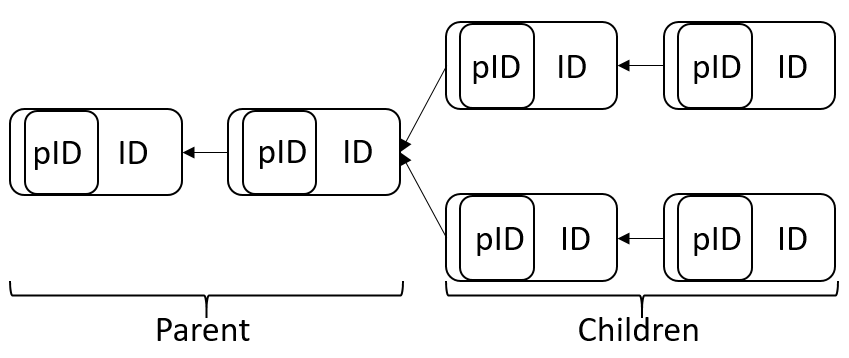
\includegraphics[scale = 0.3]{image/BlockChainStructure}
	\caption{Block chain structure is based on the tree structure: parent part is the list of blocks and children are other lists whose first blocks have the same previous ID of the last block of its parent.}
	\label{BCStructure}
\end{figure*}

\subsubsection{Adding a New Block}

\begin{figure*}[!htbp]
	\centering
%	\begin{subfigure}[b]{0.6\textwidth}
%		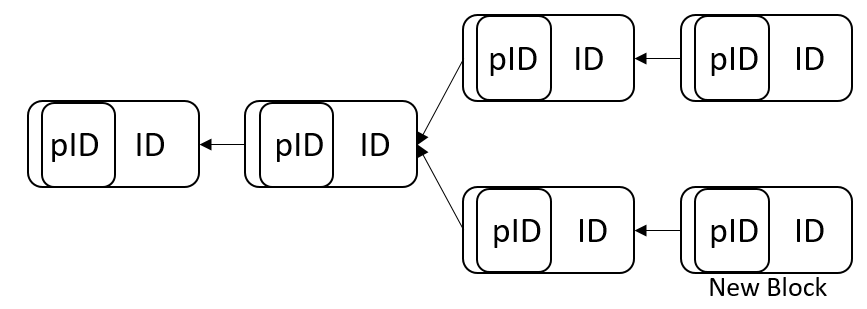
\includegraphics[scale = 0.3]{image/addB2Child}
%		\caption{Adding a new block into a child.}
%	\end{subfigure}
%	\\
	\begin{subfigure}[b]{0.6\textwidth}
		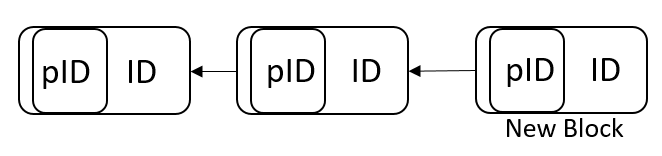
\includegraphics[scale = 0.3]{image/BC2Par}
		\caption{Adding a new block into the parent which does not have children.}
	\end{subfigure}	
	\\
	\begin{subfigure}[b]{0.6\textwidth}
		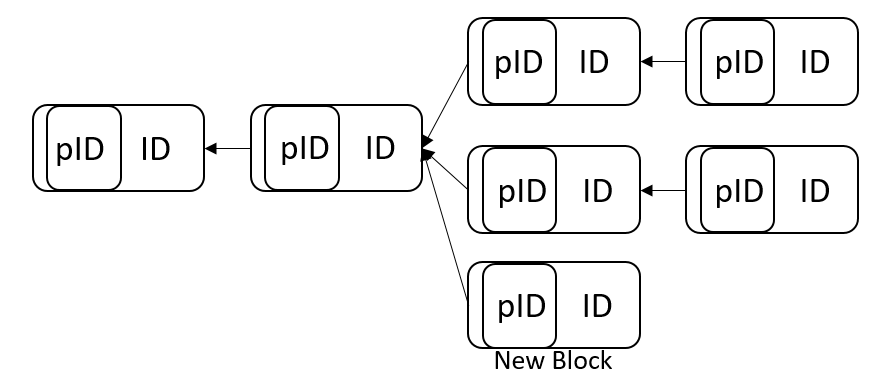
\includegraphics[scale = 0.3]{image/addB2Par3}
		\caption{Adding a new block into the end of parent which has children.}
	\end{subfigure}
	\\
	\begin{subfigure}[b]{0.6\textwidth}
		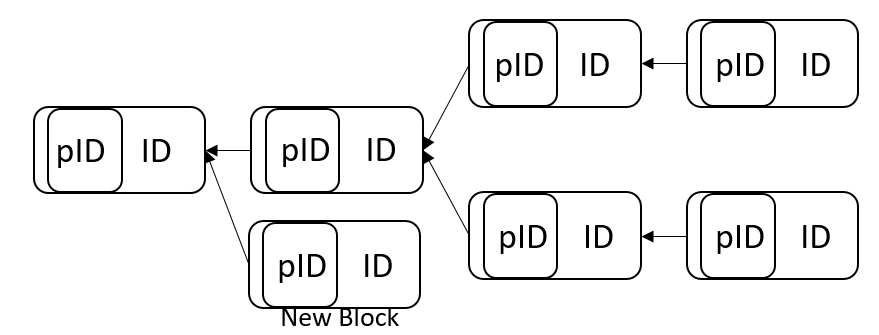
\includegraphics[scale = 0.3]{image/addB2Par2}
		\caption{Adding a new bock into the parent which has children.}
	\end{subfigure}	

	\caption{These are four cases of adding a new block in the block chain structure.}
	\label{addingBlock}
\end{figure*}

Because the block chain structure is based on the tree structure, to add a new block there are two different ways to add: adding a new block created by this node to the public chain of the same node and adding a new block received from another node to the public chain of the different node.

When a node want to create a new block, it needs to find the longest path of its public chain and then add the new block in this path.
Thus, in this case of adding a new block created and added to the block chain by the same node, the public block chain first finds the longest path to get the last block and then assigns it to the previous block of the new block.
Therefore, the new block can be created with enough fields and added to the public block chain.

On another hand, when a node want to add a new block received from another node, the public chain of the node first find the list of block which contains the previous block of the new block or the tree who contains the previous block of the new block.
After that the new block can be added to the list of block from the public chain.

Finally, the way to add a new block to a list of blocks is described by the Fig.~\ref{addingBlock} 


\section{Experiments}
\label{Exper}
In this part, the simulation is experimented with various parameters to understand the changes of number of forks and the time of consuming to solve them.



\begin{table}[!htbp]
\setlength{\tabcolsep}{10pt}			% space for cols
\renewcommand{\arraystretch}{1.5}		% space for rows
\centering
\caption{Experiments with the variety of parameters.}
\label{Experiments}
\begin{tabular}{c c c c c c c c c}
\hline
\hline
\begin{tabular}[c]{@{}c@{}}Network \\ Size \end{tabular} & \begin{tabular}[c]{@{}c@{}}No \\ Degree \end{tabular} & \begin{tabular}[c]{@{}c@{}}Selfish\\ Percent\end{tabular} & \begin{tabular}[c]{@{}c@{}}Selfish\\ Power\end{tabular} & \begin{tabular}[c]{@{}c@{}}Time of\\ 2 blocks\end{tabular} & \begin{tabular}[c]{@{}c@{}}Latency of\\ 2 nodes\end{tabular} & \begin{tabular}[c]{@{}c@{}}No \\ Forks-Avg\end{tabular} & \begin{tabular}[c]{@{}c@{}}Time Solving\\  Forks-Avg\end{tabular} \\ \cline{1-1} \hline \hline
% Net Size & NoDegree & SePercent & SePower & Time2Blocks & Latency2Nodes & NoFork       & TimeSolving

100 &  2 &  10 &  15 &  20 &  10 &  673 - 6.73 &  939 - 9.39  \\ \hline
100 &  20 &  10 &  15 &  20 &  10 &  1221 - 12.21 &  2062 - 20.62  \\ \hline
100 &  50 &  10 &  15 &  20 &  10 &  1262 - 12.62 &  2017 - 20.17  \\ \hline

100 &  2 &  50 &  70 &  20 &  10 &  433 - 4.33 &  487 - 4.87  \\ \hline
100 &  20 &  50 &  70 &  20 &  10 &  1214 - 12.14 &  2001 - 20.01  \\ \hline

100 &  2 &  1 &  1 &  20 &  10 &  695 - 6.95 &  1009 - 10.09  \\ \hline
100 &  20 &  1 &  1 &  20 &  10 &  1243 - 12.43 &  2148 - 21.48  \\ \hline

100 &  2 &  100 &  50 &  20 &  10 &  790 - 7.9 &  1051 - 10.51  \\ \hline
100 &  20 &  100 &  50 &  20 &  10 &  1232 - 12.32 &  2034 - 20.34  \\ \hline

100 &  2 &  10 &  15 &  50 &  10 &  419 - 4.19 &  427 - 4.27  \\ \hline
100 &  20 &  10 &  15 &  50 &  10 &  701 - 7.01 &  901 - 9.01  \\ \hline

%                                                          &                                                      &                                                           &                                                         &                                                          &                                                            & \begin{tabular}[c]{@{}c@{}}1000\\ 2\end{tabular}        & \begin{tabular}[c]{@{}c@{}}2000\\ 3\end{tabular}                  \\
\hline
\hline
\end{tabular}
\end{table}


From the Table~\ref{Experiments}, the first row represents about parameters while other rows illustrate different experiments from parameters.
The two last columns showing the results of the experiments are the sum of the number of forks and the amount of time to solve these forks.

With value of the table, it can be clear that with the low number of degree of each node, the number of forks and the time to consume are also low.
However, in the first three experiments, the number of degree is increasingly changed 2, 20, 50 which leads to the rise of the number of forks and the time of consuming it, but the time of consuming forks decreases in case of the number of degree equal to 50.

Another observation is when the selfish miner is 100 percent, the number of forks also increase in comparison with other case ( when the percentage of selfish miners is 50 or 10 or 1).
The last experiment can get the low number of forks because of less created blocks.
Need to note that because of these experiments based on the random functions, the results is not a perfect one.

\section{Conclusion}
\label{Con}
This assignment implements and simulates the Tinycoin, one of cryptocurrency, based on the PeerSim~\cite{jesi2005peersim} frame work with two honest and selfish~\cite{eyal2014majority} strategies.
The experiments of the simulation is implemented with PeerSim~\cite{jesi2005peersim} frame work to create a network of nodes.
After experiments, it can be clear that the number of selfish miners effect to generating forks, but the connections is the main of problem to create forks.

\section{Ackowledgements}
First and foremost, I would like to show my gratitude to Prof. Laura Ricci and her assistant PhD. Emanuele Carlini about lessons in Peer to Peer systems course. 
I also want to say thank  my classmates who supported and explained my problems through discussions and conversations,
Finally, based on the \LaTeX $ $ tool and Springer format the assignment can be completed.

\bibliography{Ref}
\bibliographystyle{plain}

\end{document}

\iffals
\begin{figure*}[t!]
	\centering
	\begin{subfigure}[b]{0.6\textwidth}
		%\centering
		
\includegraphics[scale = 0.6]{image/Unipi_Image}
		\caption{In-degree distribution with an exponent 4.5}
	\end{subfigure}
	\\
	\begin{subfigure}[b]{0.6\textwidth}
		%\centering
		
\includegraphics[scale = 0.6]{image/Unipi_Image}
		\caption{Out-degree distribution with an exponent 5.5}
	\end{subfigure}
	\caption{In-degree and Out-degree distributions}
		\label{Fig:Distri}
\end{figure*}
\textbf{Second Part}:
\begin{figure*}[t!]
	\centering
	\begin{subfigure}[b]{0.6\textwidth}
		%\centering
		
\includegraphics[scale = 0.6]{image/Unipi_Image}
		\caption{Size of WCC distribution with an exponent 10 of power law}
	\end{subfigure}
	\\
	\begin{subfigure}[b]{0.6\textwidth}
		%\centering
		
\includegraphics[scale = 0.6]{image/Unipi_Image}
		\caption{Size of SCC distribution with an exponent 9 of power law}
	\end{subfigure}

	\caption{Size of WCC and SCC distributions}
		\label{Fig:WCC_SCC}
\end{figure*}

\begin{figure*}[t!]
	\centering
	\begin{subfigure}[b]{0.6\textwidth}
		%\centering
		
\includegraphics[scale = 0.6]{image/Unipi_Image}
		\caption{Experiment with BFS on forward direction}
	\end{subfigure}
	\\
	\begin{subfigure}[b]{0.6\textwidth}
		%\centering
		
\includegraphics[scale = 0.6]{image/Unipi_Image}
		\caption{Experiment with BFS on backward direction}
	\end{subfigure}
	\\
	\begin{subfigure}[b]{0.6\textwidth}
		%\centering
		
\includegraphics[scale = 0.6]{image/Unipi_Image}
		\caption{Experiment with BFS on both directions}
	\end{subfigure}
	\caption{Experiments of BFS algorithm on three kinds of graph}
		\label{Fig:BFS}
\end{figure*}

\begin{table}[]
\centering
\caption{Experiments with the variety of parameters.}
\label{experiment}
\begin{tabular}{|c|c |c |c |c |c}
%\cline{1-1}
\hline
Size of Network               & 30          & 100           & 100           &   &  \\ \cline{1-1}
Selfish Percent               & 15          & 15            & 15            &   &  \\ \cline{1-1}
Selfish Power                 & 03          & 15            & 15            &   &  \\ \cline{1-1}
Time between 2 blocks         & 20          & 20            & 20            &   &  \\ \cline{1-1}
Latency                       & 10          & 10            & 10            &   &  \\ \cline{1-1}
Number of Degree              & 01          & 03            & 10            &   &  \\ \cline{1-1}
Number of Forks - Avg         & 22-0.73     & 1170-11.70    & 1522-15.22    &   &  \\ \cline{1-1}
Time to Solve the Forks - Avg & 2240-74.66  & 17803-178.03  & 17747-177.47  &   &  \\ %\cline{1-1}
\hline
\end{tabular}
\end{table}
